\documentclass[12pt]{beamer}

\usepackage{lmodern}
\usepackage[utf8]{inputenc}
\usepackage[T1]{fontenc}		
\usepackage[english]{babel}

\usepackage{siunitx}

\usepackage{xcolor, colortbl}
\definecolor{darkgreen}{RGB}{0, 155, 85}

\definecolor{LOSS45}{RGB}{130,8,8}
\definecolor{LOSS3545}{RGB}{183,10,10}
\definecolor{LOSS2535}{RGB}{255,0,0}
\definecolor{LOSS1525}{RGB}{255,122,12}
\definecolor{LOSS0515}{RGB}{255,181,12}
\definecolor{STBL}{RGB}{215,215,215}
\definecolor{GAIN0515}{RGB}{58,255,12}
\definecolor{GAIN1525}{RGB}{58,178,12}
\definecolor{GAIN2535}{RGB}{56,136,17}
\definecolor{GAIN3545}{RGB}{50,119,16}
\definecolor{GAIN45}{RGB}{48,83,56}


\usepackage{graphicx}
\usepackage{floatrow}
\usepackage[
    scriptsize,
    labelformat=empty
]{caption}

\usepackage{enumitem}

\usepackage{standalone}

\usepackage{multirow}

\usepackage{array}
\newcolumntype{x}[1]{>{\centering\let\newline\\\arraybackslash\hspace{0pt}}m{#1}}
\usepackage{booktabs}
\usepackage{makecell}

\usepackage{tikz}
\usetikzlibrary{calc, 3d, shadows, decorations, shapes.arrows, fadings, trees, backgrounds, fit}
\usepackage{pgfplots}
\usepackage{pgfplotstable}
\usepackage{forest}
\usepackage[final]{animate}

\usepackage{amsmath}
\usepackage{amsthm}
\usepackage{amsfonts}
\usepackage{amssymb}
\usepackage{mathrsfs}
\usepackage{bm}
\usepackage{bbold}
\usepackage{stmaryrd}
\usepackage{mleftright}
    
\usepackage[
    backend=biber,
    style=authoryear,
    dashed=false,
    sorting=nty,
    maxbibnames=5,
    minbibnames=5,
    maxcitenames=1,
    uniquelist=false,
    uniquename=false,
    hyperref=true,
    backref=true,
    backrefstyle=all+,
    isbn=false,
    url=false,
    doi=false
]{biblatex}
\usepackage{xpatch}

\addbibresource{references.bib}

\usepackage[acronym, toc, automake=true]{glossaries}

\usepackage{hyperref}
\hypersetup{
    pdftitle={Semantic aware quality evaluation of 3D building models},
    pdfauthor={Oussama Ennafii},
    pdfkeywords={3D urban modeling} {buildings} {quality assessment} {taxonomy} {classification} {error detection} {geometry} {aerial imagery} {Very High Spatial Resolution} {Digital Surface Model},
    pdfstartview={FitH},
    unicode=true
}

\setbeamerfont{footnote}{size=\tiny}

\tikzset{
    invisible/.style={opacity=0},
    visible on/.style={alt=#1{}{invisible}},
    alt/.code args={<#1>#2#3}{
        \alt<#1>{\pgfkeysalso{#2}}{\pgfkeysalso{#3}}
    },
}

\NewDocumentCommand{\evalat}{sO{\big}mm}{%
    \IfBooleanTF{#1}
    {\mleft. #3 \mright|_{#4}}
    {#3#2|_{#4}}%
}
\makeatletter
\newcommand{\ostar}{\mathbin{\mathpalette\make@circled\star}}
\newcommand{\make@circled}[2]{%
    \ooalign{$\m@th#1\smallbigcirc{#1}$\cr\hidewidth$\m@th#1#2$\hidewidth\cr}%
}
\newcommand{\smallbigcirc}[1]{%
    \vcenter{\hbox{\scalebox{0.77778}{$\m@th#1\bigcirc$}}}%
}
\makeatother


\usepackage[useregional]{datetime2}

\usepackage{style/glossaries}

\usetheme{ign}

\title{Semantic aware quality evaluation of 3D building models}
\subtitle{A scalable approach}
\date{\tiny \DTMdisplaydate{2020}{1}{10}{5}}
\author{
    Oussama Ennafii
}

\begin{document}
    \begin{frame}[plain]
        \titlepage
    \end{frame}

    \section{Introduction}
        \subsection{Context}
            \begin{frame}{\texorpdfstring{\acrshort*{acr::3d}}{3D} building model}
                \begin{itemize}[label=\(\blacktriangleright\), font=\color{IGNGreen}]
                    \item<1-> \Acrfull{acr::3d} model \(\longleftrightarrow\) generalization of the building surface.
                    \item<only@2> Surface reconstruction \(\longleftrightarrow\) geometric fidelity;
                    \item<only@3> Generalization \(\longleftrightarrow\) reduce the complexity;
                    \item<only@4> Generalization \(\implies\) \textit{implicit} semantics;
                \end{itemize}
                \onslide<2->{
                    \begin{figure}[H]
                        \centering
                        \alt<2>{
                            \includestandalone[mode=buildnew, width=.8\textwidth]{figures/model_vs_mesh/mesh_model}
                            \caption{
                                \Gls{acr::3d} mesh of a building surface (\(\approx\) \num[output-exponent-marker = \text{e}]{1e5} triangles).
                            }
                        }{
                            \includestandalone[mode=buildnew, width=.8\textwidth]{figures/model_vs_mesh/ground_truth_model}
                            \caption{
                                Building \gls{acr::3d} (polyhedral) model (\(\approx\) \num{800} facets).
                            }
                        }
                    \end{figure}
                }
            \end{frame}

            \begin{frame}{\texorpdfstring{\acrfull*{acr::lod}}{Level of Detail}}
                \begin{figure}[H]
                    \centering
                    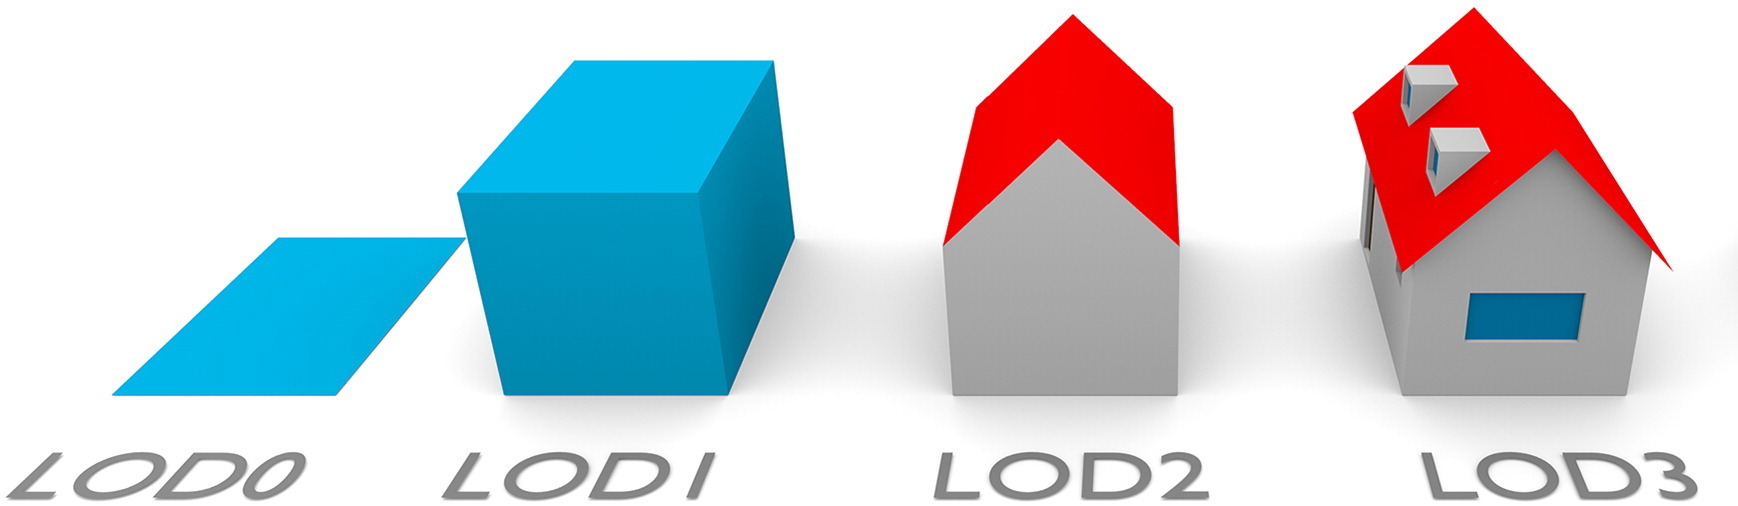
\includegraphics[width=\textwidth]{images/introduction/lods_3}
                    \caption{Considered \glspl{acr::lod}~\parencite{biljecki2016improved}.}
                \end{figure}
            \end{frame}

            \begin{frame}{Applications}
                \framesubtitle<1>{Physical simulation}
                \framesubtitle<2>{Planning}
                \framesubtitle<3>{Entertainement}

                \temporal<2>{
                    \begin{figure}[H]
                        \centering
                        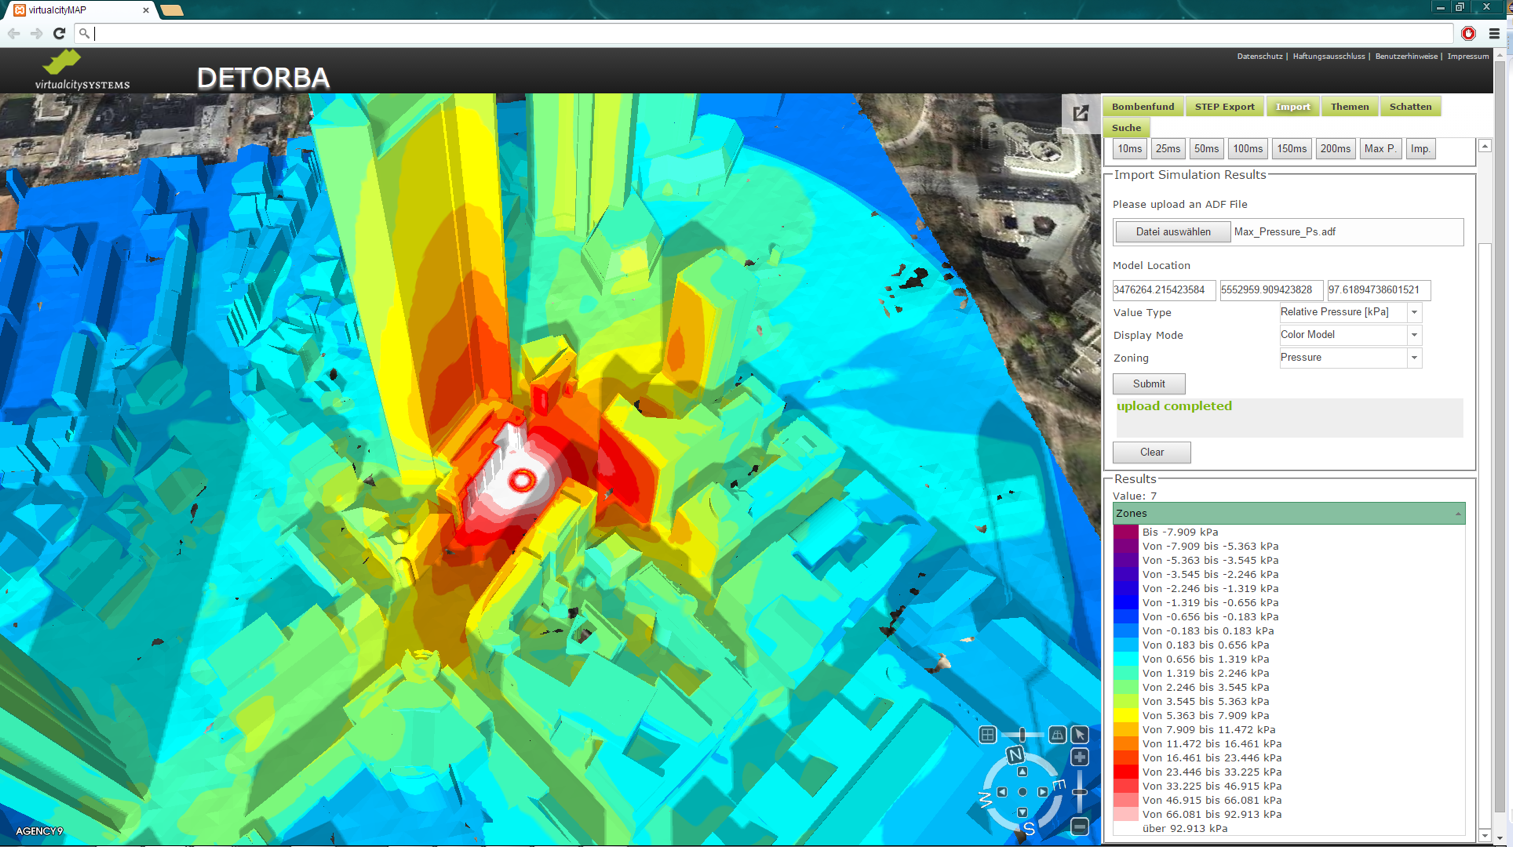
\includegraphics[width=.8\textwidth]{images/introduction/3d_model_applications/explosion_simulation}
                        \caption{Explosion simulation~\parencite{biljecki2015applications}.}
                    \end{figure}
                }
                {
                    \begin{figure}[H]
                        \centering
                        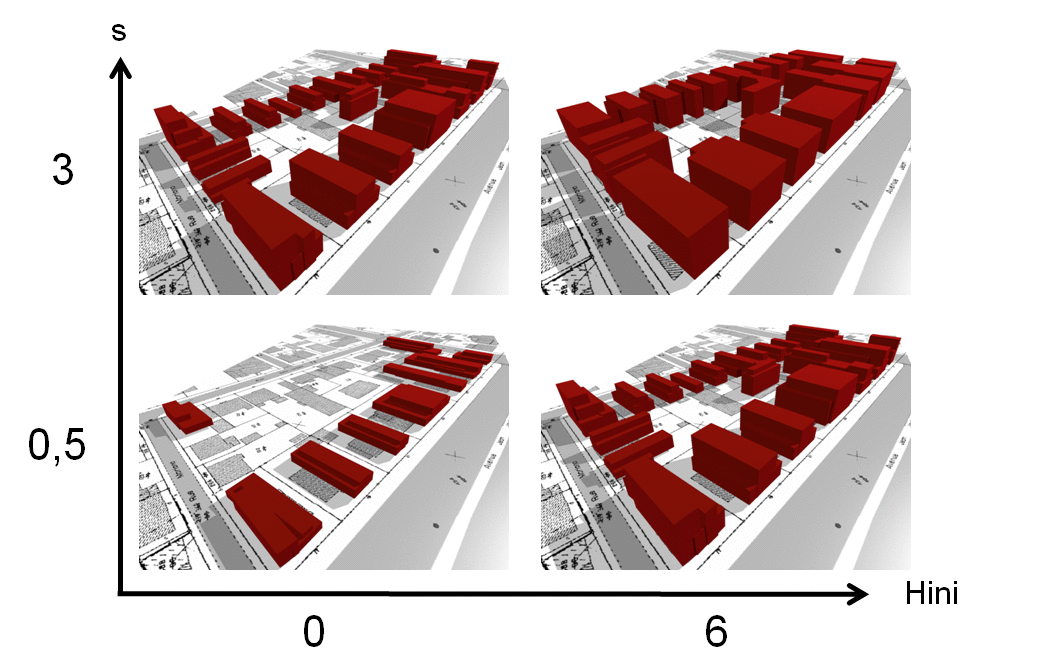
\includegraphics[width=.8\textwidth]{images/introduction/3d_model_applications/simplu}
                        \caption{Example of \gls{acr::3d} urban scene simulated based on known urban norms~\parencite{brasebin2017stochastic}.}
                    \end{figure}
                }
                {
                    \begin{figure}[H]
                        \centering
                        \animategraphics[autoplay, loop, width=.8\textwidth]{20}{images/introduction/3d_model_applications/trocadero/trocadero-}{0}{73}
                        \caption{Mixed reality for historical applications using iTowns\footnotemark platform (Credits to A. Devaux\footnotemark).}
                    \end{figure}
                    \footnotetext{
                        \href{http://www.itowns-project.org}{iTowns project.}
                    }
                    \addtocounter{footnote}{1}
                    \footnotetext{
                        \href{http://recherche.ign.fr/labos/matis/~devaux}{Alexandre Devaux website.}
                    }
                }
            \end{frame}

            \begin{frame}{\texorpdfstring{\acrshort*{acr::3d}}{3D} building modeling}
                \centering
                \includestandalone[mode=buildnew, width=\textwidth]{figures/context}
            \end{frame}

        \subsection{Motivation}
            \begin{frame}{Modeling errors}{Different point of views}
                \begin{itemize}[label=\(\blacktriangleright\), font=\color{IGNGreen}]
                    \item<1-> Errors in format: compliant to CityGML\footfullcite{ledoux2013validation} \dots.
                    \item<2-> Errors in fidelity (geometry)\uncover<2->{\footfullcite{berger2013benchmark}}.
                    \item<3-> Errors in generalization.
                \end{itemize}
            \end{frame}

            \begin{frame}{Need for semantics}
                \begin{itemize}[label=\(\blacktriangleright\), font=\color{IGNGreen}]
                    \item<1-> Modeling \(\longleftrightarrow\) compromise between:
                    \begin{itemize}[label=\(\blacktriangleright\), font=\color{IGNGreen}]
                        \item<2-> geometric accuracy;
                        \item<3-> and \textit{implicit} semantics.
                    \end{itemize}
                    \item<4-> Errors are \underline{geometric} and \underline{semantic} in nature.
                \end{itemize}
            \end{frame}
        
            \begin{frame}{State of the art}
                \centering
                \includestandalone[mode=buildnew, width=\textwidth]{figures/state_of_the_art}
            \end{frame}

            \begin{frame}{Goal}
                \begin{itemize}[label=\(\blacktriangleright\), font=\color{IGNGreen}]
                    \item<1-> \underline{Define errors} that affects building \gls{acr::3d} models.
                    \item<2-> Devise a method for \underline{error detection}.
                \end{itemize}
            \end{frame}

            \begin{frame}{Challenges}
                \begin{itemize}[label=\(\blacktriangleright\), font=\color{IGNGreen}]
                    \item<1-> Least expensive reference data;
                    \item<2-> \underline{Scalability} up to city level;
                    \item<3-> Genericity towards:
                        \begin{itemize}
                            \item<4-> modeling approach;
                            \item<5-> urban scene.
                        \end{itemize}
                    \item<6-> Automation with the least human intervention possible.
                \end{itemize}
            \end{frame}

            \begin{frame}{Contributions}
                \begin{itemize}[label=\(\blacktriangleright\), font=\color{IGNGreen}, itemsep=2em]
                    \item<1-> Semantic error taxonomy;
                    \item<2-> Learning evaluation approach;
                    \item<3-> Experimental validation.
                \end{itemize}
            \end{frame}

    \section{Semantic evaluation}
        \subsection{General layout}
            \begin{frame}{Hierarchization and Modularity}
                \begin{itemize}[label=\(\blacktriangleright\), font=\color{IGNGreen}, itemsep=2em]
                    \item<1-> Hierarchization:
                        \begin{itemize}[label=\(\blacktriangleright\), font=\color{IGNGreen}]
                            \item<2-> \underline{Iteratively} define more and more specific errors;
                            \item<3-> Each \underline{specificity level}: errors as general as possible.
                        \end{itemize}
                    \item<4-> Modularity:
                        \begin{itemize}[label=\(\blacktriangleright\), font=\color{IGNGreen}]
                            \item<5-> An error \(\equiv\) Composition of \underline{basic errors} common to all scenes.
                        \end{itemize}
                \end{itemize}
            \end{frame}
        
            \begin{frame}{Error classification}
                \includestandalone[mode=buildnew, width=\textwidth]{figures/taxonomy_tree_animated}
            \end{frame}

        \subsection{Overhead case}
            \begin{frame}{\texttt{Atomic errors}}
                \begin{itemize}[label=\(\blacktriangleright\), font=\color{IGNGreen}]
                    \item<1-> \Acrfull{acr::2d} errors:
                        \begin{itemize}[label=\(\blacktriangleright\), font=\color{IGNGreen}]
                            \item<only@2-6> Segmentation issue (semantic):
                                \begin{itemize}
                                    \item<only@3-4> Under segmentation;
                                    \item<only@5-6> Over segmentation.      
                                \end{itemize}
                            \item<only@7-11> Border issue (geometric):
                            \begin{itemize}
                                \item<only@8-9> Inaccurate topology;
                                \item<only@10-11> Imprecise border.      
                            \end{itemize}
                        \end{itemize}
                    \item<only@12-> \gls{acr::3d} error (geometric):
                        \begin{itemize}[label=\(\blacktriangleright\), font=\color{IGNGreen}]
                            \item<only@13-> Imprecise geometry.
                        \end{itemize}
                \end{itemize}
                \begin{overlayarea}{\textwidth}{.5\textheight}
                    \only<3-4>{
                        \begin{figure}[H]
                            \centering
                            \alt<3>{
                                \includestandalone[mode=buildnew, height=.4\textheight]{figures/errors/building/bos}
                                \includestandalone[mode=buildnew, height=.4\textheight]{figures/errors/building/bus}
                            }{
                                \includestandalone[mode=buildnew, height=.4\textheight]{figures/errors/facet/correct_fos_fus_fib_fig}
                                \includestandalone[mode=buildnew, height=.4\textheight]{figures/errors/facet/fus}
                            }
                            \caption{
                                \alt<3>{
                                    Ground truth buildings are in different colors: \textcolor{cyan}{blue} and \textcolor{green}{green}.
                                }{
                                    \textcolor{cyan}{Blue} \(\leftrightarrow\) under-segmented facet.
                                }
                            }
                        \end{figure}
                    }
                    \only<5-6>{
                        \begin{figure}[H]
                            \centering
                            \alt<5>{
                                \includestandalone[mode=buildnew, height=.4\textheight]{figures/errors/building/bus}
                                \includestandalone[mode=buildnew, height=.4\textheight]{figures/errors/building/bos}
                            }{
                                \includestandalone[mode=buildnew, height=.4\textheight]{figures/errors/facet/correct_fos_fus_fib_fig}
                                \includestandalone[mode=buildnew, height=.4\textheight]{figures/errors/facet/fos}
                            }
                            \caption{
                                \alt<5>{
                                    Modeled buildings are in different colors: \textcolor{cyan}{blue} and \textcolor{green}{green}.
                                }{
                                    \textcolor{green}{Green} \(\leftrightarrow\) inexisting edges.
                                }
                            }
                        \end{figure}
                    }
                    \only<8-9>{
                        \begin{figure}[H]
                            \centering
                            \alt<8>{
                                \includestandalone[mode=buildnew, height=.4\textheight]{figures/errors/building/correct_bit}
                                \includestandalone[mode=buildnew, height=.4\textheight]{figures/errors/building/bit}
                            }{
                                \includestandalone[mode=buildnew, height=.4\textheight]{figures/errors/facet/correct_fit}
                                \includestandalone[mode=buildnew, height=.4\textheight]{figures/errors/facet/fit}
                            }
                            \caption{
                                \alt<8>{
                                    \textcolor{olive}{Yellow} \(\leftrightarrow\) inaccurate borders.
                                }{
                                    \textcolor{olive}{Yellow} \(\leftrightarrow\) inaccurate borders.
                                }
                            }
                        \end{figure}
                    }
                    \only<10-11>{
                        \begin{figure}[H]
                            \centering
                            \alt<10>{
                                \includestandalone[mode=buildnew, height=.4\textheight]{figures/errors/building/correct_bib}
                                \includestandalone[mode=buildnew, height=.4\textheight]{figures/errors/building/bib}
                            }{
                                \includestandalone[mode=buildnew, height=.4\textheight]{figures/errors/facet/correct_fos_fus_fib_fig}
                                \includestandalone[mode=buildnew, height=.4\textheight]{figures/errors/facet/fib}

                            }
                            \caption{
                                \alt<10>{
                                    \textcolor{red}{Red} \(\leftrightarrow\) imprecise borders.
                                }{
                                    \textcolor{red}{Red} \(\leftrightarrow\) imprecise borders.
                                }
                            }
                        \end{figure}
                    }
                    \only<13-14>{
                        \begin{figure}[H]
                            \centering
                            \alt<13>{
                                \includestandalone[mode=buildnew, height=.4\textheight]{figures/errors/building/correct_big}
                                \includestandalone[mode=buildnew, height=.4\textheight]{figures/errors/building/big}
                            }{
                                \includestandalone[mode=buildnew, height=.4\textheight]{figures/errors/facet/correct_fos_fus_fib_fig}
                                \includestandalone[mode=buildnew, height=.4\textheight]{figures/errors/facet/fig}
                            }
                            \caption{
                                \alt<12>{
                                    \textcolor{violet}{Purple} \(\leftrightarrow\) imprecise facet.
                                }{
                                    \textcolor{violet}{Purple} \(\leftrightarrow\) imprecise facet geometry.
                                }
                            }
                        \end{figure}
                    }
                \end{overlayarea}
            \end{frame}

    \section{Learned evaluation}
        \begin{frame}{Evaluation is classification}
            \begin{itemize}[label=$\blacktriangleright$, font=\color{IGNGreen}]
                \item<1-> Evaluation at \underline{building level};
                \item<2-> Error detection \(\leftrightarrow\) supervized classification;
                \item<3-> Respects both constraints:
                    \begin{itemize}[label=$\blacktriangleright$, font=\color{IGNGreen}]
                        \item<4-> \textbf{Large-scale}: prediction on unseen instances;
                        \item<5-> \textbf{Automation}: needs manual annotations.
                    \end{itemize}
            \end{itemize}
        \end{frame}

        \begin{frame}{The evaluation pipeline}
            \begin{figure}[H]
                \includestandalone[mode=buildnew, height=.75\textheight]{figures/graphical_pipeline}
            \end{figure}
        \end{frame}

        \subsection{Baseline}
            \begin{frame}{Geometric features}
                \centering
                \includestandalone[mode=buildnew, width=.75\textwidth]{figures/features/geometric_animated}
            \end{frame}

            \begin{frame}{Height based features}
                \centering
                \includestandalone[mode=buildnew, width=\textwidth]{figures/features/height_based_animated}
            \end{frame}

            \begin{frame}{Image based features}
                \centering
                \includestandalone[mode=buildnew, height=.8\textheight]{figures/features/image_based_animated}
            \end{frame}

        \subsection{Advanced graph features}
            \begin{frame}{Random walk on graphs}
                \begin{figure}[H]
                    \caption{Random walk on graph \(G\).}
                    \alt<1>{
                        \centering
                        \animategraphics[autoplay, loop, width=.45\textwidth]{25}{figures/features/drunk_man/drunk_man-}{0}{72}
                        \includestandalone[mode=buildnew, width=.45\textwidth]{figures/features/random_walk}
                    }{
                        \centering
                        \includestandalone[mode=buildnew, width=.45\textwidth]{figures/features/random_walk}
                    }
                \end{figure}
                \begin{itemize}[label=\(\blacktriangleright\), font=\color{IGNGreen}]
                    \item<4-> Described \(\longrightarrow\) normalized adjacency matrix \(P\);
                    \item<5-> \(P\) as a feature vector \(\longrightarrow\) \pause \alert<6->{No};
                    \item<7-> \(P\) is not \underline{invariant} to:
                    \begin{itemize}
                        \item<8-> permutations;
                        \item<9-> graph size.
                    \end{itemize}
                    \item<10-> Kernel trick \(\longrightarrow\) \pause compare graphs instead.
                \end{itemize}
            \end{frame}

            \begin{frame}{Random walk based kernels}
                \framesubtitle<1-4>{Random walk kernel}
                \framesubtitle<5-13>{Multiscale Laplacian kernel}
                \framesubtitle<14->{Propagation kernel}
                \only<1-4>{
                    \begin{columns}[T]
                        \centering
                        \begin{column}{.4\textwidth}
                            \centering
                            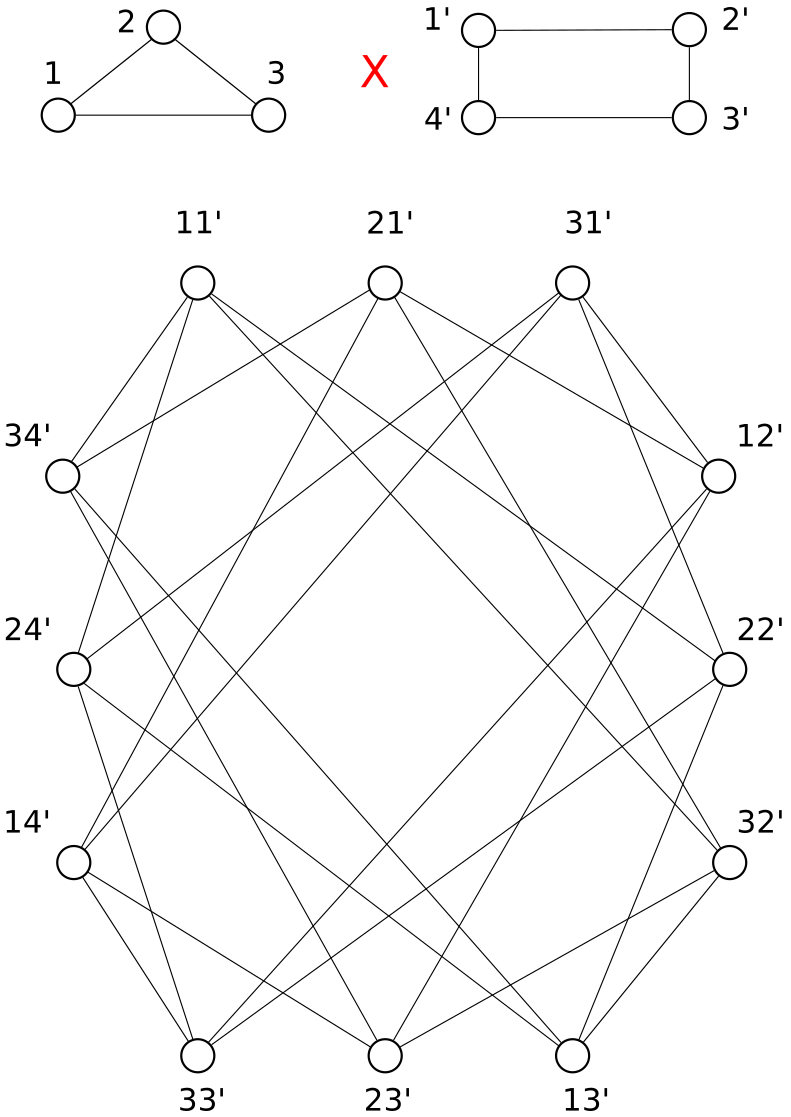
\includegraphics[width=\textwidth]{images/related_work/direct_product_graphs}
                        \end{column}
                        \begin{column}{.56\textwidth}
                            \centering
                            \begin{itemize}[label=\(\blacktriangleright\), font=\color{IGNGreen}]
                                \item<2-> Quadratic form with \(P_{\times}\) \(\implies\) \underline{invariance} to:
                                    \begin{itemize}[label=\(\blacktriangleright\), font=\color{IGNGreen}]
                                        \item<3-> permutation;
                                        \item<4-> graph size;
                                    \end{itemize}
                            \end{itemize}
                        \end{column}
                    \end{columns}
                }
                \only<5-13>{
                    \vfill
                    \begin{itemize}[label=\(\blacktriangleright\), font=\color{IGNGreen}]
                        \item<5-> \(G\) \(\longleftrightarrow\) Variance matrix of a Gaussian distribution.
                        \item<6-> Compare graphs \(\longrightarrow\) Compare probabilities.
                        \item<7-> Adapted to be:
                        \begin{itemize}[label=\(\blacktriangleright\), font=\color{IGNGreen}]
                            \item<8-> permutation and size invariant \(\longrightarrow\) \pause linear embedding;
                            \item<10-> node attribute aware \(\longrightarrow\) \pause vertex kernel Gram matrix;
                            \item<12-> Scalability \(\longrightarrow\) \pause kernel between pyramid of subgraphs.
                        \end{itemize}
                    \end{itemize}
                    \vfill
                }
                \only<14->{
                    \begin{itemize}[label=\(\blacktriangleright\), font=\color{IGNGreen}]
                        \item<14-> Nodes are Gaussian mixtures of other nodes;
                        \item<15-> Propagate mixture coefficients using \(P\);
                        \item<16-> Probability distributions are hashed \(\longrightarrow\) \pause graph feature vector.
                    \end{itemize}
                }
            \end{frame}

            \begin{frame}{Graph Hopper kernel}
                \begin{overlayarea}{\textwidth}{.5\textheight}
                    \only<1>{
                        \begin{figure}[H]
                            \centering
                            \caption{Tottering: \textcolor{purple!30}{isolated} nodes are less visited.}
                            \includestandalone[mode=buildnew, width=.45\textwidth]{figures/features/tottering}
                        \end{figure}
                    }
                    \only<2->{
                        \centering
                        \includestandalone[mode=buildnew, width=\textwidth]{figures/features/graph_hopper}
                    }
                \end{overlayarea}
                \begin{itemize}[label=\(\blacktriangleright\), font=\color{IGNGreen}]
                    \item<2-> Compare \underline{paths} instead (no cycles);
                    \begin{itemize}[label=\(\blacktriangleright\), font=\color{IGNGreen}]
                        \item<3-> Sum over same length paths.
                        \item<6-> Hop and compare vertex attributes \(\longrightarrow\) base kernel.
                        \item<10-> Sum over all vertex comparisons \(\longrightarrow\) \underline{invariance}.
                    \end{itemize}
                \end{itemize}
            \end{frame}

            \begin{frame}{Lov\'asz/\texorpdfstring{\acrshort*{acr::svm}}{SVM} kernel}
                \begin{itemize}[label=\(\blacktriangleright\), font=\color{IGNGreen}]
                    \item<1-> Lov\'asz number \(\vartheta\left(G\right)\):
                    \begin{itemize}[label=\(\blacktriangleright\), font=\color{IGNGreen}]
                        \item<2-3> graph invariant;
                        \item<3> smallest cone containing the orthonormal representation of \(G\).
                    \end{itemize}
                    \item<4-> Compare graphs \(\longleftrightarrow\) Compare Lov\'asz number of subgraphs.
                    \item<5-> \(\vartheta\left(G\right)\) not easy to compute \(\longleftrightarrow\) Approximation with \gls{acr::svm} kernel.
                \end{itemize}
            \end{frame}

            \begin{frame}{Advanced graph features}
                \centering
                \includegraphics{example-image}
            \end{frame}

        \subsection{Advanced image features}
            
            \begin{frame}{\texorpdfstring{\acrshort*{acr::scatnet}}{ScatNet}}
                \begin{itemize}[label=\(\blacktriangleright\), font=\color{IGNGreen}]
                    \item<1-> Reverse engineered \acrfull{acr::cnn};
                    \item<2-> Ingredients: 
                    \begin{itemize}[label=\(\blacktriangleright\), font=\color{IGNGreen}]
                        \item<3-> Band pass filters \(\longrightarrow\) high frequency information;
                        \item<4-> Modulus \(\longrightarrow\) non-linearity;
                        \item<5-> Average pooling operator \(\longrightarrow\) invariance.
                    \end{itemize}
                \end{itemize}
            \end{frame}
            
            \begin{frame}{\texorpdfstring{\acrshort*{acr::scatnet}}{ScatNet} structure}
                \centering
                \includestandalone[mode=buildnew, width=\textwidth]{figures/scattering_network_animated}
            \end{frame}

            \begin{frame}{\texorpdfstring{\acrshort*{acr::scatnet}}{ScatNet} filters}
                \centering
                \alt<2>{
                    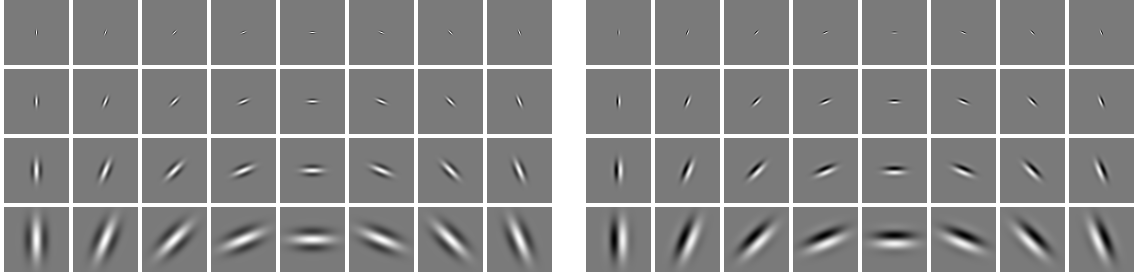
\includegraphics[width=\textwidth]{images/related_work/morlet_wavelets}
                }
                {
                    
\includegraphics[width=.5\textwidth]{images/related_work/first_layer_cnn}\\
                    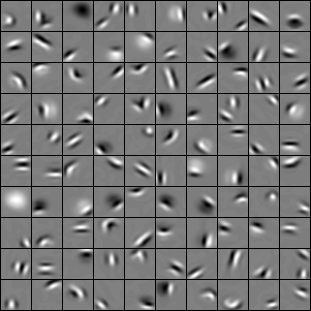
\includegraphics[width=.75\textwidth]{images/related_work/second_layer_cnn}
                }
            \end{frame}

            \begin{frame}{Advanced height based features}
                \centering
                \includestandalone[mode=buildnew, width=\textwidth]{figures/features/height_based_scatnet}
            \end{frame}

            \begin{frame}{Advanced image based features}
                
            \end{frame}

    \section{Experiments}
        \begin{frame}{Datasets: urban scenes}
            \centering
            \includestandalone[mode=buildnew, width=.9\textwidth]{figures/dataset}
        \end{frame}
        
    \section{Conclusion}
        \begin{frame}{\textcolor{yellow}{Conclusion} \& \textcolor{purple}{Perspectives}}
            \begin{itemize}[label=\(\blacktriangleright\), font=\color{yellow}, itemsep=2em]
                \item<1-> \textbf{Hierarchical and modular} taxonomy;
                \item<2-> \textbf{Fast, lightweight and modular} pipeline for model evaluation;
                \item<3-> Pipeline tested with \textbf{baseline} and \textbf{advanced} handcrafted features:
                    \begin{itemize}[label=\(\blacktriangleright\), font=\color{IGNGreen}]
                        \item<4-> Geometric features are often sufficient for error prediction;
                        \item<5-> Adding modalities is most helpfull for transferability.
                    \end{itemize}
            \end{itemize}
            \uncover<6->{
                ~\\
                Future work:
                \begin{itemize}[label=\(\blacktriangleright\), font=\color{purple}, itemsep=2em]
                    \item<6-> Use of deep learning.
                    \item<7-> Dataset augmentation $\longrightarrow$ \textbf{Simulate errors}.
                \end{itemize}
            }
        \end{frame}
\end{document}
